\chapter{Networks of Drones}
In this chapter we begin with what an unmanned aerial vehicle (UAV) is and the degrees of autonomy drones can have. Then we walk through the networks of drones — how multiple UAVs cooperate, what a “dronet” is, and the practical problems that researchers and engineers care about. 

\section{Unmanned Aerial Vehicle (UAV)}
A \textit{UAV} is simply an aircraft that flies without a human pilot on board (see Figure \ref{fig:uav}). This vehicle may operate with various degrees of autonomy: at one extreme a human on the ground directly pilots every motion via remote control; at the other extreme the aircraft makes all decisions onboard (like sensing, planning and acting) without human intervention.

\begin{figure}[ht]
    \centering
    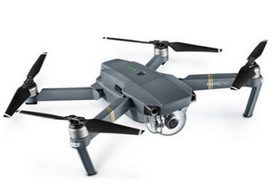
\includegraphics[height=0.174\linewidth]{images/uav1.png}
    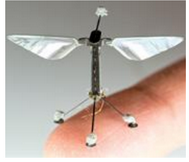
\includegraphics[height=0.174\linewidth]{images/uav2.png}
    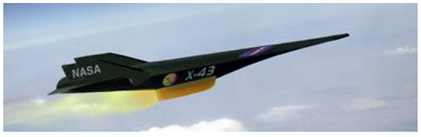
\includegraphics[height=0.174\linewidth]{images/uav3.png}
    \caption{Types of UAV.}
    \label{fig:uav}
\end{figure}

When we say “autonomy” we mean the ability of the drone to sense its environment and take decisions without continuous human input. This can be only partial (e.g., automatic takeoff/landing or waypoint following) or full mission autonomy (find, track and act on targets by itself). 
Drones vary enormously in size, capability and endurance, and those differences shape how they are used.
To give a sense of the extremes: tiny research prototypes can weigh less than a gram, while very large high-altitude military drones weigh many tonnes. Speed also spans a wide range: hobby and commercial quadcopters typically cruise at tens to a few hundreds kilometers per hour, whereas some experimental unmanned hypersonic vehicles reached many thousands of kilometers per hour. Propulsion and energy are fundamental constraints. Fuelled propulsion (gasoline, methane, hydrogen) gives long endurance and higher speeds but adds complexity, emissions and maintenance. Electric propulsion dominates small and medium commercial drones because batteries (Ni-Cd, Ni-MH, Li-Po, and emerging Li-S) are light, quiet and easy to manage; the trade-off is flight time. Solar cells are sometimes used to extend endurance for high-altitude, long-duration platforms.

Finally, drones come in different mechanical forms: single-rotor helicopters, multi-rotor (quad, hexa, octo), fixed-wing airplanes and lighter-than-air platforms like airships. Each form has trade-offs: multi-rotors hover and offer high maneuverability at the cost of energy efficiency, while fixed-wing designs are efficient for covering long distances but need forward speed to stay aloft.

Drones bring a few advantages that explain why they are being widely adopted. 
First, they can be deployed quickly and reach areas that are otherwise inaccessible, which is invaluable in disaster response. They can carry small but critical payloads — medical supplies, sensors or communications equipment — to places where roads are blocked or dangerous. They reduce human exposure to hazardous environments, whether that’s a collapsed building, wildfire perimeter or polluted site.
Beyond emergencies, drones are useful for everyday tasks such as traffic monitoring, wind estimation for meteorology and remote sensing for agriculture or infrastructure inspection. Their flexibility and relatively low cost make them appealing for many sensing and monitoring roles.

\section{Dronet}
When multiple UAVs operate together in the same area and coordinate, we call that a \textit{dronet} or UAV network (see Figure \ref{fig:dronet}). The point of a dronet is cooperation: drones share sensor data, plan their movements to avoid overlap, forward mission-critical information, and sometimes act as flying communications infrastructure.

\begin{figure}[ht]
    \centering
    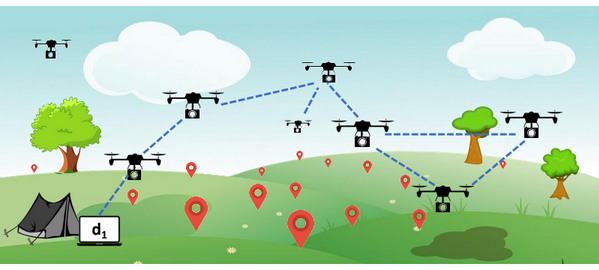
\includegraphics[width=0.7\linewidth]{images/dronet.png}
    \caption{Dronet.}
    \label{fig:dronet}
\end{figure}

Imagine an area of interest where several drones are flying. Some might be focused on sensing while others form a communication backbone to move the sensed data back to a control station. Often there is also a depot or control center on the ground that owns the mission and may provide higher level commands.

In many scenarios, successful operation requires drones to exchange substantial amounts of data: high-resolution images, video streams, telemetry, position and status updates, maps and mission plans. Designing networks that move this data efficiently and reliably is one of the main engineering challenges.

There are four central issues in dronets:
\begin{enumerate}
    \item How to provide communication in emergency scenarios where there is no network infrastructure available? After storms, earthquakes or in very remote areas, cellular towers and wired backhaul may be down or non-existent.
    \item How to optimize task assignment and trajectory planning for UAVs operating in real-world scenarios? Each drone has limited battery, limited payload and physical motion constraints. The planner must assign which drone does which job and compute paths that respect these limits while minimizing time, energy or mission risk.
    \item How to perform continuous data offloading when deployed in large and harsh areas? Continuous offloading is when drones stream data as they collect it.
    \item How to perform periodic data offloading when deployed in large and harsh areas? Periodic offloading is when drones store data locally for some time and only upload when they rendezvous with a depot or come into contact with a stronger link.
\end{enumerate}

\subsection{How do we provide communication in emergency situations where there is no network infrastructure?}
Drones can act as flying base stations, temporarily providing wireless access to users on the ground. They can act as relay nodes that bridge line-of-sight gaps, forming a mobile mesh that routes traffic from isolated teams to the internet or a control hub. They can act as backhaul nodes: a high-altitude drone can link a cluster of lower drones to a satellite or a fixed ground station.

Always remember the constraints: limited battery, payload, regulatory restrictions, weather sensitivity, and the cost/complexity of operation. The higher the autonomy and the more integrated the networking capability, the more complex the onboard software becomes and the heavier the energy burden. That’s why mission design usually involves trade-offs: fewer sensors and more flight time, or richer sensing at the cost of frequent returns to the depot.

As case study the DANGER system from the academic literature: “DANGER: a Drone-Aided Network for Guiding Emergency and Rescue operations,” authored by Andrea Coletta, Gaia Maselli, Mauro Piva and Domenicomichele Silvestri, is an example of research that tackles the problem of using drones to provide on-the-spot communications for emergency response.

\subsection{How to optimize task assignment and trajectory planning for UAVs operating in real-world scenarios?}
That short description hides a lot. Let’s translate it into what you actually need to think about.
\begin{enumerate}
    \item \textit{“Multi-depot”} means drones don’t all start or charge from one fixed point. In an emergency, some drones might be based at a vehicle, others at a rooftop depot, and yet others at a temporary field base. That affects how you route drones between missions and where they can refill energy or offload data.
    \item \textit{Squads} and \textit{heterogeneity} means that some drones carry thermal cameras and must hover to acquire useful frames; others are relay drones with larger batteries but limited sensing; some can carry extra batteries or replacement radios. Assign the right drone to the right trajectory and the right task.
    \item The \textit{“set of trajectories”} formulation is important because in many deployments you predefine mission patterns — sweep lines, circular loitering trajectories, or orbiting paths around a site — and select which of those predefined patterns each drone will fly.
    \item The \textit{“required target hovering time”} means each target imposes a minimum dwell time before the drone can be considered to have completed its sensing or communications goal.
\end{enumerate}

\subsection{How to perform continuous data offloading when deployed in large and harsh areas?}
When drones carry sensors they produce data that must reach the depot or operators.
Continuous offloading means streaming data as it is collected, such as a video feed streamed from a search drone to a command vehicle. Continuous offload requires low latency and sustained bandwidth. This typically implies either line-of-sight wideband links (e.g., Wi-Fi at short range, directional links) or relayed multi-hop connections where drones forward data along a chain to a gateway drone with a backhaul (satellite or ground link).

Dronets (UAVNETs) look similar to wireless sensor networks or MANETs, but they change the game in several ways.
Mobility in drone networks is medium to high, and it can be three-dimensional. Topologies are fluid; drones move, hover, leave for recharging and reappear. Node failure is common either because of batteries, hardware faults or collisions. Energy is constrained and often the single most important resource. Crucially, moving a drone typically costs far more energy than sending a modest radio packet. These characteristics affect every networking layer.

\subsubsection{MAC}
Drones commonly carry multiple radio modules depending on mission needs. Wi-Fi is a common choice because it’s widely supported by user devices and offers wide bandwidth at short ranges. Cellular can provide robust backhaul and mobility support, but in many emergency or remote scenarios cellular connectivity is not available. Low Power Wide Area Networks like LoRa give long range and low energy consumption, but they offer tiny bandwidth and are inappropriate for high-rate video.

\subsubsection{Routing}
Routing in dronets is driven by the need to stream wideband content from moving drones back to a depot. Large-area monitoring may require multihop connections because a single wideband link seldom covers the whole area. The question is “which routing protocol?”

Comparing classical Wireless Sensor Networks to dronets makes the differences clear. WSN nodes are usually static or mildly mobile, energy harvesting might be available, and the topology is relatively stable. Dronets are highly mobile in 3D, topologies are fluid, nodes fail more often, and the mission contexts include rescue and surveillance with strict real-time demands.

Because of these differences, routing goals change. In dronets we care about keeping overhead low, guaranteeing loop freedom, ensuring scalability as the number of drones grows, conserving energy, reducing delay especially for high-priority traffic, and increasing delivery ratio under mobility.

\begin{itemize}
    \item \textit{Proactive protocols} keep tables of routes to every other node and periodically refresh them. The advantage is that routes are immediately available when you need them. The downside is control traffic overhead and slow convergence under very high mobility; keeping route tables consistent across fast-moving nodes is expensive and can cause stale information. For these reasons, plain proactive protocols often struggle in high-mobility dronets unless carefully tuned.
    
    Examples to be aware of are OLSR (Optimized Link State Routing), DSDV (Destination Sequenced Distance Vector), and B.A.T.M.A.N. OLSR runs periodic hello and topology control messages and uses multipoint relays to reduce flooding. DSDV is a distance-vector protocol with sequence numbers to prevent loops. B.A.T.M.A.N. is also categorized as proactive but it actually uses a different philosophy: it distributes link quality information and only stores next-hop choices, reducing the need for global knowledge.
    \item \textit{Reactive protocols} discover routes on demand, so they avoid periodic control traffic at rest but incur discovery latency when communication starts. In highly dynamic scenarios, frequent discoveries can themselves overwhelm the network. Typical reactive protocols are DSR and AODV.
    \item \textit{Hybrid protocols} try to get the best of both worlds by making route discovery proactive inside a local zone and reactive beyond it. This reduces discovery delays locally while limiting global overhead. ZRP and TORA are classic hybrids, but hybrid protocols can be hard to implement and tune in practice.
    \item \textit{Geographic protocols} take a different approach: they route using node positions rather than full route tables. If nodes know their positions and the destination’s approximate location, a node can forward to a neighbor closer to the destination. Drones typically have GPS and position information, and it naturally adapts to mobility. However, it requires location knowledge and suffers around voids or obstacles in the network where greedy forwarding fails; fallback strategies are needed.
\end{itemize}

\paragraph{B.A.T.M.A.N}
B.A.T.M.A.N., short for \textit{Better Approach To Mobile Ad-hoc Networking}, is a lightweight, decentralized mesh routing protocol. Unlike classical link-state protocols that try to build a global view, B.A.T.M.A.N. keeps things local: each node learns only which neighbor is the best next hop for reaching a certain originator. That simple decision reduces the amount of global state each node keeps.
    
\begin{enumerate}
    \item Each node periodically broadcasts an \textit{Originator Message} or OGM that identifies itself. Neighbors forward OGMs so they propagate through the network. 
    \item OGMs contain a sequence number so that nodes can determine which OGMs are fresh and avoid routing loops or replayed old information. 
    \item Nodes evaluate how often they receive OGMs from a neighbor as a proxy for link quality: if you receive OGMs frequently and with low loss, that neighbor likely offers a good path to that originator. 
    \item Based on these observations, each node records the best next hop toward each originator in a small table.
\end{enumerate}
Let’s break down the contents of a typical OGM packet: 
The originator address is simply the identifier of the node that sent the OGM; the sequence number timestamps and orders OGMs to avoid mistaken use of old reports; the Time-to-Live (TTL) limits hops so OGMs don’t propagate indefinitely; the Link Quality indicator (LQ) may be explicit or derived from how many OGMs are received and how recent they are, it gives a measure of the stability and reliability of the link between the neighbor and the originator; the hop count is useful for path length estimation and sometimes used for route selection.

\paragraph{Asymetric links}
Imagine two drones, \texttt{A} and \texttt{B} (see Figure \ref{fig:asymmetric-link}). \texttt{A} shouts its presence by sending periodic Originator Messages (OGMs). \texttt{B} hears \texttt{A} clearly and receives every OGM. But when \texttt{B} talks, \texttt{A} receives almost nothing. The radio behavior is asymmetric: packets reliably flow from \texttt{A} to \texttt{B}, but not from \texttt{B} to \texttt{A}.

\begin{figure}
    \centering
    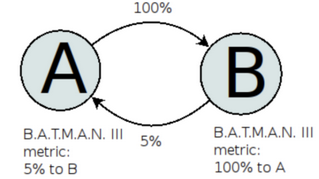
\includegraphics[width=0.4\linewidth]{images/asymmetric-link.png}
    \caption{Asymmetric link.}
    \label{fig:asymmetric-link}
\end{figure}

This asymmetry is a real headache for routing algorithms that infer link quality by counting received control packets. If you simply count how many OGMs you get from a neighbor, \texttt{B} will conclude the link from \texttt{A}$\to$ \texttt{B} is near perfect (it receives lots of OGMs). But that measurement says nothing about the opposite direction, \texttt{B}$\to$ \texttt{A}. If \texttt{B} uses only that count to advertise “I have a great link to \texttt{A}”, it’s lying — from \texttt{A}’s point of view, the link is poor.
So the system needs a way to detect and correct for asymmetry: not just “how many OGMs do I receive from you?” but also “how many of my OGMs do you forward (or otherwise reflect) back to me?” \textit{B.A.T.M.A.N. IV} solves this using two related but distinct counters: \textit{Receive Quality} and \textit{Echo Quality}, and combines them into a \textit{Transmit Quality} metric.

\begin{itemize}
    \item If node \texttt{A} looks at how many OGMs from \texttt{B} arrived in the last \texttt{N} seconds, that count (often normalized into a 0–1 fraction) is \texttt{A}’s estimate of \texttt{B}$\to$ \texttt{A} link reliability (see Figure \ref{fig:receive-quality}). 
    
    \begin{figure}[ht]
        \centering
        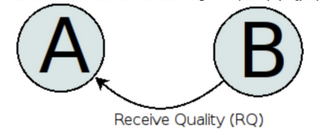
\includegraphics[width=0.4\linewidth]{images/receive-quality.png}
        \caption{Receive quality.}
        \label{fig:receive-quality}
    \end{figure}
    
    We often write this as:
    \begin{equation*}
        RQ = \textit{number of OGMs received from neighbor (within sliding window)}
    \end{equation*}
    So if \texttt{B} sent 100 OGMs in the window and \texttt{A} received 90, \texttt{A}’s RQ for \texttt{B} is 0.90. That tells \texttt{A} how good the neighbor$\to$ me direction has been, but it doesn’t tell \texttt{A} whether its own transmissions reach the neighbor.
    \item \textit{Echo Quality} is the clever bit that helps detect asymmetry. The intuition is simple: if I broadcast OGMs, do my neighbors rebroadcast them in such a way that I can observe those rebroadcasts? If yes, that indicates the neighbor actually heard my OGMs and is willing (and able) to forward them — i.e., my transmissions reach them.

    Concretely, EQ can be implemented by counting how many times the neighbor rebroadcasts OGMs that originated from you. You detect that because OGMs include the originator address and sequence numbers. When you later hear a neighbor forwarding an OGM that lists you as originator, that’s an “echo” of your own packet (see Figure \ref{fig:echo-quality}).

    \begin{figure}[ht]
        \centering
        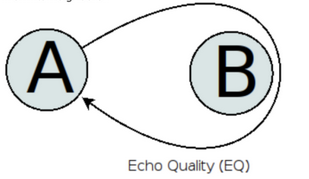
\includegraphics[width=0.4\linewidth]{images/echo-quality.png}
        \caption{Echo quality.}
        \label{fig:echo-quality}
    \end{figure}

    So EQ is effectively:
    \begin{equation*}
        EQ = \textit{number of times neighbor rebroadcasts your OGMs (within sliding window)}
    \end{equation*}
    If many of your OGMs are echoed back by the neighbor, your transmission toward that neighbor is likely successful.

    \item To produce a usable bidirectional link estimate, B.A.T.M.A.N. IV computes \textit{Transmit Quality} as the ratio of echo counts to receive counts. One practical formula is:
    \begin{equation*}
        TQ = EQ / RQ        
    \end{equation*}
    RQ tells you how many OGMs you heard from the neighbor (their transmissions toward you). EQ tells you how many of your OGMs the neighbor admitted to rebroadcasting (an indirect signal that your transmissions reached them). If RQ is large but EQ is small, you are in the asymmetric case where you receive their OGMs but they don't reliably receive yours — TQ becomes small and that link is demoted. If both EQ and RQ are high, TQ approaches 1 and the link is symmetric and good.
\end{itemize}

Suppose in the last sliding window:
    \begin{itemize}
        \item Node \texttt{B} counted RQ\_B(A) = 80 OGMs received from \texttt{A} (out of an expected 100), so RQ $\approx$ 0.80.
        \item Node \texttt{B} also observed that A’s OGMs were rebroadcast by \texttt{B} (and heard back) only 40 times, so EQ $\approx$ 0.40.
    \end{itemize}   
Then \texttt{B} would compute TQ $\approx$ EQ/RQ = 0.40 / 0.80 = 0.5. That TQ of 0.5 tells \texttt{B} that while it seems to hear \texttt{A} often, \texttt{A} likely doesn’t hear \texttt{B} reliably — the effective two-way usability of the link is moderate at best.

B.A.T.M.A.N. also uses a clever propagation mechanism so that nodes can estimate the end-to-end transmit quality to an originator through multiple hops. The idea is multiplicative: when an OGM is forwarded, each forwarding node multiplies the incoming TQ by its own local link quality and writes the result into the packet before rebroadcast.

Start by having the originator broadcast with a maximum TQ field (think of this as 1.0). A direct neighbor that receives it measures its local TQ to the originator (based on EQ/RQ or a local LQ estimate) and multiplies:
\begin{equation*}
    TQ\_outgoing = TQ\_incoming \times TQ\_local    
\end{equation*}
So if node \texttt{A} sets $TQ\_incoming$ = 1.0 when sending, node \texttt{B} receives and computes $TQ\_local(B\iff A) = 0.8$; \texttt{B} rebroadcasts the OGM carrying $TQ = 1.0 \times 0.8 = 0.8$. Node \texttt{C} receives that rebroadcast, measures its own $TQ\_local(C\iff B) = 0.9$, and rebroadcasts with $TQ = 0.8 \times 0.9 = 0.72$. The TQ that \texttt{C} carries for originator \texttt{A} (0.72) now reflects the cumulative product of local link qualities across the path \texttt{A}$\to$ \texttt{B}$\to$ \texttt{C}. Any node seeing an OGM learns not only that \texttt{A} exists, but also a scalar estimate of how well \texttt{A}’s transmissions are likely to arrive at that node (see Figure \ref{fig:transmit-quality-propagation}).

\begin{figure}[ht]
    \centering
    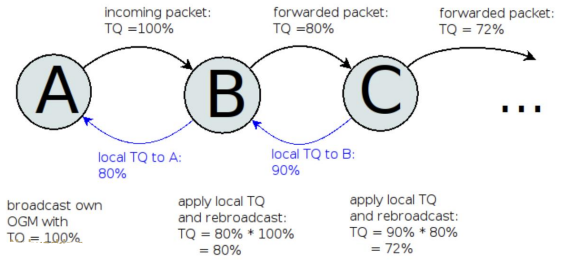
\includegraphics[width=0.7\linewidth]{images/transmit-quality-propagation.png}
    \caption{Transmit quality propagation.}
    \label{fig:transmit-quality-propagation}
\end{figure}

This multiplicative scheme has a strong intuitive property: long weak chains produce small TQ numbers, and short strong links produce larger TQs. It gives nodes a compact, end-to-end metric without requiring full path knowledge.

\paragraph{Geographic routing}
Every drone knows its own position — usually via GPS — and periodically exchanges position beacons with neighbors. When a node has a packet to forward to a destination, it looks up the destination’s coordinates and forwards the packet to the neighbor whose position is closest to the destination. That greedy step repeats until the packet reaches the destination.

Geographic routing has two big advantages for dronets. First, it uses only local information (your neighbors’ positions) so it scales well and adapts to mobility. Second, it avoids route discovery overhead: there is no table of whole-path routes to maintain.

Drones operate in three dimensions, so the routing decision should use 3-D Euclidean distance. \textit{GDSTR-3D} (Geographic Distance-based STRategy in 3D) picks the neighbor with minimal 3-D distance to the destination.
This approach is simple, but it can fail. A packet can arrive at a node that has no neighbor closer to the destination than itself. That node is in a \textit{dead end} or local minimum (see Figure \ref{fig:dead-ends}). In 2-D sensor networks researchers devised techniques to route around obstacles by walking the edges of a planar subgraph. With drones, the situation is easier because drones can move. If a node is at a dead end, you might reposition one or more drones for a few seconds to break the dead end.


In geographic routing there are three simple strategy to handle the forwarding decisions:
\begin{itemize}
    \item \textit{Greedy forwarding.} When a node must forward a packet, it hands the packet to the neighbor whose position is closest (in Euclidean distance) to the destination (see Figure \ref{fig:greedy-forwarding}). Then that neighbor repeats the rule. It’s cheap, needs no route discovery and stores no big tables, but it suffers from the local-optimum (dead-end) problem: you can get stuck at a node that is the closest so far yet has no neighbor closer to the destination.

    \begin{figure}[ht]
        \centering
        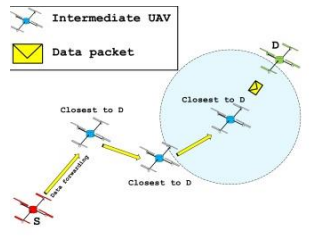
\includegraphics[width=0.5\linewidth]{images/greedy-forwarding.png}
        \caption{Greedy forwarding.}
        \label{fig:greedy-forwarding}
    \end{figure}
    
    \item \textit{Store-carry-and-forward.} If connectivity is not continuous, a node simply keeps the packet, moves (or continues its mission), and forwards the data later when it meets a suitable relay or gets within range of the depot (see Figure \ref{fig:store-carry-forward}). This is the delay-tolerant networking mindset and it works well when latency requirements are loose and mobility is predictable or favorable.

    \begin{figure}[ht]
        \centering
        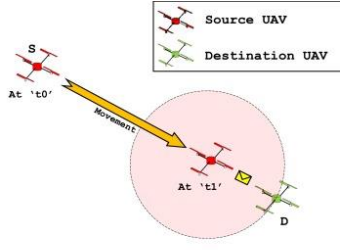
\includegraphics[width=0.5\linewidth]{images/store-carry-forward.png}
        \caption{Store-carry and forward.}
        \label{fig:store-carry-forward}
    \end{figure}
    
    \item \textit{Prediction.} Here you use position plus heading and speed to forecast future locations of neighbors (see Figure \ref{fig:prediction}). Forwarding decisions favor nodes that not only are close now but are likely to remain useful (or become even better) shortly. Prediction reduces pointless handovers and helps avoid fleeting contacts that won't actually progress the packet.

    \begin{figure}[ht]
        \centering
        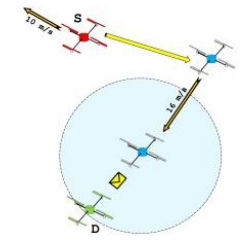
\includegraphics[width=0.4\linewidth]{images/prediction.png}
        \caption{Prediction forwarding.}
        \label{fig:prediction}
    \end{figure}
\end{itemize}

\subsection{How to perform periodic data offloading when UAVs are deployed in large and harsh areas?}
You have a squad of UAVs performing sensing over a large area and a depot where collected data must be offloaded. Offloading uses a short-range, high-data-rate channel like Wi-Fi, so UAVs must get physically near the depot (or a connected UAV) to dump large payloads. Each UAV has localization (GPS), and the area may be too large for constant connectivity.

The design goal is to periodically build a connected topology so data can be offloaded while also: 
minimizing the extra distance UAVs must travel to form that topology, minimizing the time needed to form the connected topology, and maximizing the time UAVs spend on their sensing mission (see Figure \ref{fig:periodic-connectivity-problem}).

\begin{figure}[ht]
    \centering
    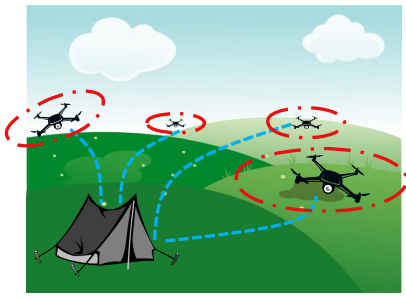
\includegraphics[width=0.5\linewidth]{images/periodic-connectivity-problem.png}
    \caption{Periodic connectivity problem.}
    \label{fig:periodic-connectivity-problem}
\end{figure}

\subsubsection{Stop \& Route}
The \textit{Stop \& Route} solution (Novella Bartolini et al., WONS 2023) tackles the periodic offloading problem with a distributed protocol that avoids global planning. The idea is simple and pragmatic: discretize the area, have UAVs exchange lightweight heartbeats and hello beacons, and use a Follow-Leader mechanism so that a connected chain of UAVs forms on demand between remote nodes and the depot. Some UAVs become stationary relays (they STOP) while others follow leaders to fill connectivity gaps.

Important assumptions for the distributed version (see Figure \ref{fig:stop-route1}): the operational area is discretized into tiles or rendezvous points, high-data-rate offloading uses short-range Wi-Fi only, UAVs are lazy-synchronized, the depot periodically transmits heartbeat packets so nearby UAVs, UAVs periodically send hello messages to advertise position and state, and a Follow-Leader mechanism lets UAVs form connected chains by following a closer-to-depot UAV that acts as a leader.

\begin{figure}[ht]
    \centering
    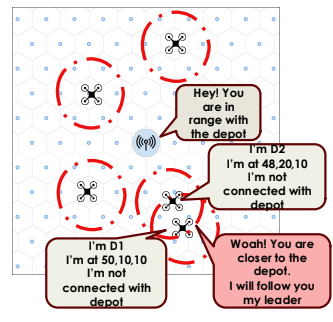
\includegraphics[width=0.5\linewidth]{images/stop-route1.png}
    \caption{Stop \& route distributed solution.}
    \label{fig:stop-route1}
\end{figure}

This lightweight signaling is enough for UAVs to locally decide whether to stop and act as part of the offload chain, follow another UAV, or keep sweeping their sensing area.

DGA is the core local rule set used by Stop \& Route during the “connected formation building” phase.
Each UAV repeatedly evaluates three conditions (see Figure \ref{fig:stop-route2}):
\begin{itemize}
    \item If it is in direct communication range of the depot, or if it is connected to another UAV that itself can reach the depot, then it stops — it will act as a stationary relay or offload node. Stopping means holding position on a tile and serving as part of the connected topology.
    \item If it sees a non-connected UAV that is closer to the depot than itself, it adopts a follow-leader role: it sets that neighbor as its leader and moves to follow it, effectively marching the chain toward the depot.
    \item If it is isolated — no connected neighbor and no closer node in range — it keeps moving along its mission toward the rendezvous point that is the next tile closer to the depot.
\end{itemize}

\begin{figure}[ht]
    \centering
    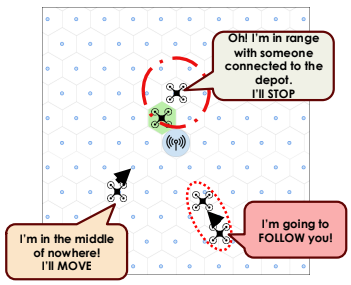
\includegraphics[width=0.5\linewidth]{images/stop-route2.png}
    \caption{Stop \& route distributed gathering algorithm (DGA).}
    \label{fig:stop-route2}
\end{figure}

\begin{Example}{Stop \& Route – DGA}{}
Think of the area as a grid of tiles. The depot sits at some tile near one edge. Initially most UAVs keep moving along their own sensing trajectories. When a UAV (call it \texttt{D1}) comes into Wi-Fi range of the depot, it stops and becomes a connected tile. Nearby UAVs that hear \texttt{D1} and are not yet connected check whether they are closer to the depot than the UAVs they hear; if so one becomes a follower and moves to the tile right behind \texttt{D1}, then stops itself, creating a two-hop chain. Meanwhile other UAVs that are farther keep advancing toward the next rendezvous tile. Step by step the chain grows, but only as large as necessary to bridge the gap.

\begin{minipage}{\textwidth}
    \centering
    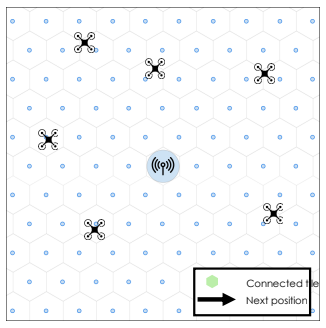
\includegraphics[width=0.34\linewidth]{images/stop-route-ex1.png}
    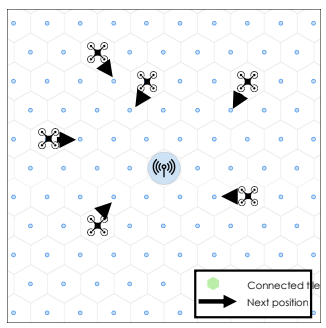
\includegraphics[width=0.34\linewidth]{images/stop-route-ex2.png}
    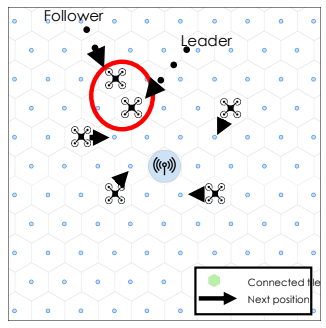
\includegraphics[width=0.34\linewidth]{images/stop-route-ex3.png}
    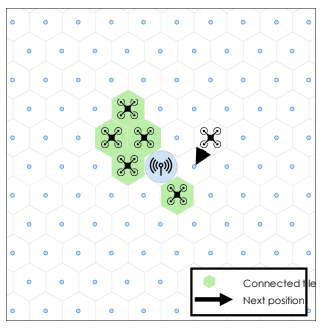
\includegraphics[width=0.34\linewidth]{images/stop-route-ex4.png}
    %\captionsetup{hypcap=false}
    %\captionof{figure}{Query tree.}
    \label{fig:stop-route-ex}
\end{minipage}
\end{Example}

Stop \& Route’s strength is its low-communication, fully distributed nature and the fact that it minimizes unnecessary movement by only having the minimal set of UAVs stop and form the chain.
